\let\negmedspace\undefined
\let\negthickspace\undefined
\documentclass[journal]{IEEEtran}
\usepackage[a5paper, margin=10mm, onecolumn]{geometry}
\usepackage{lmodern} % Ensure lmodern is loaded for pdflatex
\usepackage{tfrupee} % Include tfrupee package

\setlength{\headheight}{1cm} % Set the height of the header box
\setlength{\headsep}{0mm}  % Set the distance between the header box and the top of the text

\usepackage{csquotes}
\usepackage{gvv-book}
\usepackage{gvv}
\usepackage{circuitikz}
\usepackage{cite}
\usepackage{amsmath,amssymb,amsfonts,amsthm}
\usepackage{algorithmic}
\usepackage{graphicx}
\usepackage{textcomp}
\usepackage{xcolor}
\usepackage{txfonts}
\usepackage{listings}
\usepackage{enumitem}
\usepackage{mathtools}
\usepackage{gensymb}
\usepackage{comment}
\usepackage[breaklinks=true]{hyperref}
\usepackage{tkz-euclide} 
\usepackage{listings}
% \usepackage{gvv}                                        
\def\inputGnumericTable{}                                 
\usepackage[latin1]{inputenc}                                
\usepackage{color}                                            
\usepackage{array}                                            
\usepackage{longtable}                                       
\usepackage{calc}                                             
\usepackage{multirow}                                         
\usepackage{hhline}                                           
\usepackage{ifthen}                                           
\usepackage{lscape}
\usepackage{caption}
\usepackage{tikz}
\usetikzlibrary{patterns}
\begin{document}

\bibliographystyle{IEEEtran}

\begin{center}
    \textbf{\Large GATE 2008\\
    AGRICULTURAL ENGINEERING (AG)\\
    MAIN PAPER}
\end{center}

\bigskip


\textbf{Duration:} Three Hours \hfill \textbf{Maximum Marks:} 150

\textbf{Q.1-Q.20 carry one mark each}

\medskip
\begin{enumerate}
\item 
 If $f(x)$ is a perfect normal distribution with mean and standard deviation of 5 and 1 respectively, then the value of $f(x)$ for $x = 6$ is
\begin{enumerate}
\begin{multicols}{4}
\item 0.124
\item 0.242
\item 0.482
\item 0.524
\end{multicols}
\end{enumerate}
\hfill(GATE AG 2008)\\

\medskip

\item 
 Eigenvalues of the matrix
 \myvec{ 
 2 & 1 \\
 2 & 3 \\
 } are 
\begin{enumerate}
\begin{multicols}{4}
\item 1 and 2
\item 1 and 3
\item 1 and 4
\item 2 and 3 
\end{multicols}
\end{enumerate}
\hfill(GATE AG 2008)\\

\medskip

\item  
 
$ \int_0^{\pi/2} \frac{\cos \theta }{\sqrt{1 - \cos^2 \theta}} d\theta $ is 
\begin{enumerate}
\begin{multicols}{4}
\item  0  
\item  $\frac{\pi}{2}$ 
\item  1 
\item  $\pi$
\end{multicols}
\end{enumerate}
\hfill(GATE AG 2008)\\

\medskip

\item 
 A function $f(x)$ is evaluated as 1, 1.5, 2.2 and 3.4 at four values of $x$ having intervals of 0.5. The area under the curve $f(x)$ using trapezoidal rule is 
\begin{enumerate}
\begin{multicols}{4}
 \item 1.95
 \item 2.45
 \item 2.95
 \item 3.45
 \end{multicols}
 \end{enumerate}
 \hfill(GATE AG 2008)\\

\medskip


\item
 If $\log_e(y) = -x \log_e(x)$, then the maximum value of $y$ is 
\begin{enumerate}
\begin{multicols}{4}
 \item e 
 \item $e^{x^2}$ 
 \item $e^{e^{-1}}$ 
 \item $e^x$ 
\end{multicols}
\end{enumerate}
\hfill(GATE AG 2008)


\medskip

\item 
 The cross product of $\mathbf{x} = 2\mathbf{i}+\mathbf{j}$ and $\mathbf{y} = \mathbf{i}-2\mathbf{j}+\mathbf{k}$ is 
\begin{enumerate}
\begin{multicols}{2}
\item  $\mathbf{i}-\mathbf{j}+2\mathbf{k}$
\item  $\mathbf{i}-2\mathbf{j}+5\mathbf{k}$
\item  $\mathbf{i}-2\mathbf{j}-5\mathbf{k}$
\item  $2\mathbf{i}-4\mathbf{j}$
\end{multicols}
\end{enumerate}
\hfill(GATE AG 2008)\\

\medskip

\item 
 Inverse Laplace Transform of $\frac{1}{(s-2)^2}$ is 
\begin{enumerate}
\begin{multicols}{4}
\item  $e^{2t}$
\item  $t e^{2t}$
\item  $2t e^{t}$
\item  $t^2 e^{2t}$
\end{multicols}
\end{enumerate}
\hfill(GATE AG 2008)\\

\medskip

\item 
 Solution of the ordinary differential equation 
 \begin{align}
\frac{dy}{dx} = x^2 + 2y  
 \end{align} is
\begin{enumerate}
\begin{multicols}{2}
\item  $y = \frac{2}{3} x^2 + 4x$
\item  $y = \sqrt{\frac{2}{3} x^2 + 4x + k}$
\item  $y = \frac{2}{3} x^3 - 4x + k$
\item  $y = \frac{2}{3} x^3 + 4x + k$
\end{multicols}
\end{enumerate}
\hfill(GATE AG 2008)\\

\medskip

\item 
 The area of a map plotted to a scale of 1:3000 measures $9069.37$ mm$^2$. The 20 m chain used for this survey was short by 0.2 m. The true land area it represents is \\
\begin{enumerate}
\begin{multicols}{4}
\item  83281 m$^2$
\item  82449 m$^2$
\item  80808 m$^2$
\item  80000 m$^2$
\end{multicols}
\end{enumerate}
\hfill(GATE AG 2008)\\

\medskip

\item 
 To measure the difference in level precisely between two points with a leveling instrument having collimation error, the method to be used is 
\begin{enumerate}
\begin{multicols}{2}
\item  reciprocal leveling
\item  check leveling
\item  compound leveling
\item  profile leveling
\end{multicols}
\end{enumerate}
\hfill(GATE AG 2008)\\

\medskip

\item 
 Three catchments A, M and F each having an area of 10,000 km$^2$ are situated in an arid zone, mountainous region of a temperate zone and flat region of a temperate zone respectively. The desirable number of hydrometeorological stations for these three catchments, $N_A$, $N_M$ and $N_F$, respectively will be such that 
\begin{enumerate}
\begin{multicols}{2}
\item  $N_M > N_F > N_A$
\item  $N_A < N_M < N_F$
\item  $N_A > N_M > N_F$
\item  $N_M = N_F$ and $N_M > N_A$
\end{multicols}
\end{enumerate}
\hfill(GATE AG 2008)\\

\medskip

\item 
 The following design parameters of contour bunds constructed on a land of 4\% slope are given: V.I. = 1.2 m, base width = 2.5 m, top width = 0.5 m, height = 1.0 m. Assuming the length for side and lateral bunds as 30\% of the length of contour bunds, the land area lost due to bunding is 
\begin{enumerate}
\begin{multicols}{4}
\item  0.156\%
\item  2.50\%
\item  10.83\%
\item  12.52\%
\end{multicols}
\end{enumerate}
\hfill(GATE AG 2008)\\

\medskip

\item 
 The percentage of husk, bran and bran oil received from rice milling are respectively 
\begin{enumerate}
\begin{multicols}{2}
\item  20, 5 and 25
\item  5, 10 and 30
\item  20, 5 and 40
\item  20, 10 and 20
\end{multicols}
\end{enumerate}
\hfill(GATE AG 2008)\\

\medskip

\item 
 In order to freeze a fruit juice its thermodynamic temperature is 
\begin{enumerate}
\item  higher than the freezing point of water
\item  below the freezing point of water
\item  equal to the freezing point of water
\item  dependent upon the water content of the fruit juice 
\end{enumerate}
\hfill(GATE AG 2008)\\

\medskip

\item 
 When a suspension of microorganism is heated at constant temperature, the reaction kinetics of decrease in the number of the organism is 
\begin{enumerate}
\begin{multicols}{4}
\item  linear
\item  exponential
\item  parabolic
\item  hyperbolic
\end{multicols}
\end{enumerate}
\hfill(GATE AG 2008)\\

\medskip

\item 
 Water activity ($a_w$) is a ratio of 
\begin{enumerate}
\item  vapour pressure of water to partial pressure of water in the product
\item  partial pressure of water in air to partial pressure of air at saturation
\item  vapour pressure of water in equilibrium with the food to vapour pressure of pure water at the same temperature 
\item  vapour pressure of pure water to vapour pressure of water in equilibrium with food
\end{enumerate}
\hfill(GATE AG 2008)\\

\medskip

\item 
 Two links OA and OB are connected by a pin joint at O such that $\angle$AOB is $144^ \degree$. If the diameter of pin joint is $d$ and the angular velocity of each link is $\omega$, then the velocity of rubbing at the pin joint O when the links move in opposite directions is 
\begin{enumerate}
\begin{multicols}{4}
\item  0
\item  $\omega d$
\item  $\frac{2}{5} \pi \omega d$ 
\item  $\frac{1}{2}\omega d$
\end{multicols}
\end{enumerate}
\hfill(GATE AG 2008)\\

\medskip

\item 
 The essential requirement for turning in a power tiller is accomplished by having 
\begin{enumerate}
\item  both the wheels as towed wheels
\item  only one wheel driven by the engine, while the other wheel is always free to rotate
\item  one of the wheels disconnected from the engine at the time of turning
\item  the same mechanism as used in a rear wheel driven tractor
\end{enumerate}
\hfill(GATE AG 2008)\\

\medskip

\item 
 The function of a differential lock used in a rear wheel driven tractor is 
\begin{enumerate}
\item  to operate both the rear wheels at the same speed 
\item  to operate both the rear wheels at differential speeds 
\item  to operate both the rear wheels at the same torque 
\item to evenly distribute the power to both the wheels 
\end{enumerate}
\hfill(GATE AG 2008)\\

\medskip

\item
 The nature of variation of tractive efficiency (TE) with wheel slip (S) in a rear wheel driven tractor is \\
\begin{figure}[h]
    \centering
    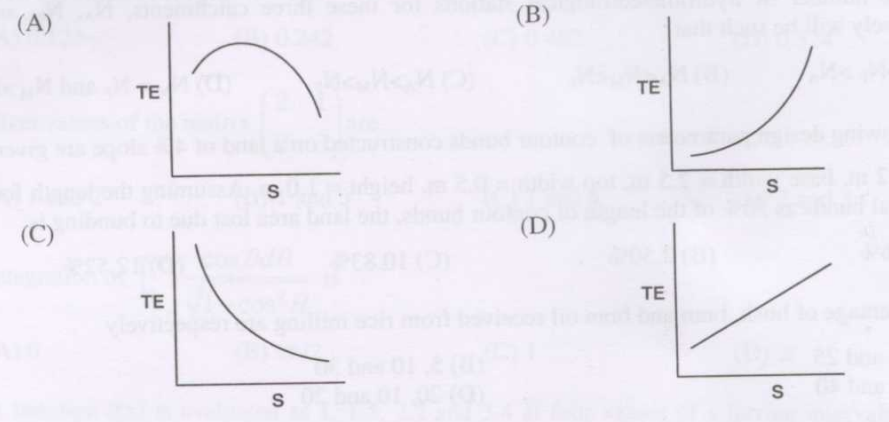
\includegraphics[width=0.7\columnwidth]{Figs/Screenshot 2025-08-07 170331.png}
    \caption{}
    \label{fig 1}
\end{figure}
\hfill(GATE AG 2008)


\medskip


Q.\,21 to Q.\,75 carry two marks each.

\bigskip

\item 
 The correlation analysis between $X$ and $Y$ variables assuming the parabolic relationship revealed a nonlinear correlation coefficient of $0.98$. The percentage of the total variation that remains unexplained by assuming a parabolic relationship between $X$ and $Y$ is
\begin{enumerate}
\begin{multicols}{4}
\item  $2.0$
\item  $96.0$
\item  $3.96$
\item  $10.0$
\end{multicols}
\end{enumerate}
\hfill(GATE AG 2008)\\

\medskip

\item 
  Cycloid is formed by $x = a(\theta-\sin\theta)$ and $y = a(1-\cos\theta)$. The surface area of the curved plane obtained from the rotation of the cycloid around $x$ axis is
\begin{enumerate}
\begin{multicols}{4}
\item  $16\pi a^2$
\item  $\frac{32\pi a^2}{3}$
\item  $\frac{64\pi a^2}{3}$
\item  $\frac{128\pi a^2}{3}$
\end{multicols}
\end{enumerate}
\hfill(GATE AG 2008)\\

\medskip

\item 
 If one bucket contains $8$ red balls and $2$ black balls and another bucket contains $7$ red balls and $3$ black balls, the probability of having at least one red ball from drawings of one ball from each of the two buckets is
\begin{enumerate}
\begin{multicols}{4}
\item  $0.94$
\item  $0.84$
\item  $0.56$
\item  $0.38$
\end{multicols}
\end{enumerate}
\hfill(GATE AG 2008)\\

\medskip

\item 
 In a factory $30\%$ of the machines are assembled by robots and $70\%$ are assembled by manual labour. Reliability of the first type of machines is $0.9$ and that of the second type of machines is $0.8$. One piece of machine was found to be reliable. The probability of the machine having been assembled by robot is
\begin{enumerate}
\begin{multicols}{4}
\item  $0.325$
\item  $0.565$
\item  $0.675$
\item  $0.835$
\end{multicols}
\end{enumerate}
\hfill(GATE AG 2008)\\

\medskip

\item 
 If  $\sum_{i=1}^n (x - a_i)^2$ has a minima at $A$, then $A$ is the arithmetic mean of the series
\begin{enumerate}
\begin{multicols}{2}
\item  $a_1 - a_2 + a_3 - \ldots + (-1)^{n+1} a^n$
\item  $ \frac{1}{a_1} + \frac{1}{a_2} + \frac{1}{a_3} + \ldots + \frac{1}{a_n}$
\item  $ \frac{1}{a_1} - \frac{1}{a_2} + \frac{1}{a_3} - \ldots + (-1)^{n+1} \frac{1}{a_n}$
\item  $a_1 + a_2 + a_3 + \ldots + a_n$
\end{multicols}
\end{enumerate}
\hfill(GATE AG 2008)\\

\medskip

\item 
 Solution of the differential equation 
\[\frac{dy}{dx} - 7y = e^x \quad \text{is}\]
\begin{enumerate}
\begin{multicols}{2}
\item $e^x(Ce^{6x} - 6^{-1})$
\item $e^{7x}(e^{-6x} - C)^{-1}$
\item $e^x(Ce^{-6x} - 6^{-1})$
\item $e^x[C e^x + (6e^x)^{-1}]$
\end{multicols}
\end{enumerate}
\hfill(GATE AG 2008)\\

\medskip

\item 
 A clayey soil has a field capacity of $0.38\ \text{m}^3/\text{m}^3$ and wilting point of $0.24\ \text{m}^3/\text{m}^3$. If the specific weight of the soil is $12.75\ \text{kN/m}^3$ and the effective root-zone depth is $0.8$ m, the available moisture holding capacity is
\begin{enumerate}
\begin{multicols}{4}
\item $15.6$ cm
\item $11.2$ cm
\item $1.12$ cm
\item $20.8$ cm
\end{multicols}
\end{enumerate}
\hfill(GATE AG 2008)\\

\medskip

\item 
 A flow of $150\ \text{L s}^{-1}$ was supplied for 8 hours from a tank to irrigate 2 ha of land. It was found that the actual delivery rate at the farm was less than $150\ \text{L s}^{-1}$. If the conveyance loss was $864$ m\textsuperscript{3} and percolation and runoff losses in the field were 240 and 760 m\textsuperscript{3} respectively, the water application efficiency of this system is
\begin{enumerate}
\begin{multicols}{4}
\item 80\%
\item 61\%
\item 77\%
\item 71\%
\end{multicols}
\end{enumerate}
\hfill(GATE AG 2008)\\

\medskip

\item 
 The following data were obtained from an agricultural land requiring a pipe drainage system for groundwater control:
\begin{itemize}
\item Hydraulic conductivity = 8.3 cm/h
\item Drainable porosity = 5\%
\item Reaction factor = 0.31 per day
\item Equivalent depth to the impermeable layer = 2.8 m
\end{itemize}

The drain spacing computed by the Glover-Dumm formula will be
\begin{enumerate}
\begin{multicols}{4}
\item 60 m
\item 190 m
\item 50 m
\item 6 m
\end{multicols}
\end{enumerate}
\hfill(GATE AG 2008)\\

\medskip

\item 
 A tile drainage system draining 12 ha flows at the design capacity for two days in response to a storm. If the system is designed using a drainage coefficient of 1.25 cm, the amount of water removed from the drainage area during two days is
\begin{enumerate}
\begin{multicols}{4}
\item $150\ \text{m}^3$
\item $1500\ \text{m}^3$
\item $30\ \text{m}^3$
\item $3000\ \text{m}^3$
\end{multicols}
\end{enumerate}
\hfill(GATE AG 2008)\\

\medskip

\item 
 The analysis of maximum one-day rainfall in a city indicated that a depth of 280 mm has a return period of 50 years. The probability of a one-day rainfall depth equal to or greater than 280 mm in the city occurring two times in 15 successive years is
\begin{enumerate}
\begin{multicols}{4}
\item 0.032
\item 0.323
\item 0.042
\item 0.272
\end{multicols}
\end{enumerate}
\hfill(GATE AG 2008)\\

\medskip

\item 
 A catchment with an area of 756 km\textsuperscript{2} has a 6 h unit hydrograph which is triangular with a base of 70 h. The peak discharge of direct runoff hydrograph due to 5 cm of rainfall excess in 6 h from the catchment is
\begin{enumerate}
\begin{multicols}{4}
\item $60\ \text{m}^3/\text{s}$
\item $535\ \text{m}^3/\text{s}$
\item $300\ \text{m}^3/\text{s}$
\item $756\ \text{m}^3/\text{s}$
\end{multicols}
\end{enumerate}
\hfill(GATE AG 2008)\\

\medskip

\item 
 A 50 g L\textsuperscript{-1} solution of a tracer was discharged into a stream at a constant rate of 20 mL s\textsuperscript{-1}. At a downstream section, the tracer was completely mixed and the concentration was measured as 10 parts per billion. Assuming the background concentration as zero, the stream discharge is
\begin{enumerate}
\begin{multicols}{4}
\item $100\ \text{m}^3/\text{s}$
\item $200\ \text{m}^3/\text{s}$
\item $800\ \text{m}^3/\text{s}$
\item $1000\ \text{m}^3/\text{s}$
\end{multicols}
\end{enumerate}
\hfill(GATE AG 2008)\\

\medskip

\item 
 The velocity of flow of water through a drop inlet pipe spillway is 4 m s\textsuperscript{-1} and the friction loss coefficient is 0.12. Maximum slope that can be provided to the pipe to maintain pipe flow condition is
\begin{enumerate}
\begin{multicols}{4}
\item 8.9\%
\item 9.8\%
\item 10.3\%
\item 10.8\%
\end{multicols}
\end{enumerate}
\hfill(GATE AG 2008)\\

\medskip

\item 
 If $W$ is the width of a bench terrace constructed on a land of slope $S$, then the drop ($D$) between two consecutive bench terraces for a riser slope of $1/2 : 1$ is given by
\begin{enumerate}
\begin{multicols}{4}
\item $D = \frac{WS}{100 - S}$
\item $D = \frac{WS}{200 - S}$
\item $D = \frac{2WS}{200 - S}$
\item $D = \frac{2WS}{100 - S}$
\end{multicols}
\end{enumerate}
\hfill(GATE AG 2008)\\

\medskip

\item 
 A centrifugal pump delivers $0.03\ \text{m}^3/\text{s}$ of water through a 100 mm diameter pipe to a vertical height of 14 m from the centerline of the pump. The pump is installed 6.0 m above water level in the sump and the head loss in the pipeline is found to be 5 m of water. If the overall efficiency is 72\%, the power required to run the pump will be
\begin{enumerate}
\begin{multicols}{4}
\item 7.36 kW
\item 10.22 kW
\item 8.18 kW
\item 5.89 kW
\end{multicols}
\end{enumerate}
\hfill(GATE AG 2008)\\

\medskip

\item 
 A double acting single cylinder reciprocating pump has a cylinder diameter of 150 mm and stroke 300 mm. Suction and delivery heads for the pump are 3.0 and 30 m respectively. If the pump delivers $0.01033\ \text{m}^3/\text{s}$ of water at 60 rpm, the percentage slip is
\begin{enumerate}
\begin{multicols}{4}
\item 97.43
\item 1.57
\item 2.57
\item 0.0257
\end{multicols}
\end{enumerate}
\hfill(GATE AG 2008)\\

\medskip

\item 
 In the Moody diagram, the third parameter is $\varepsilon/D$. Here, $\varepsilon$ is
\begin{enumerate}
\item the equivalent uniform sand grain roughness
\item an arbitrarily chosen roughness magnitude
\item median size in a non-uniform sand grain roughness
\item mean height of the actual roughness of commercial pipes
\end{enumerate}
\hfill(GATE AG 2008)\\

\medskip

\item 
 Atmospheric pressure at a place is equal to 10 m of water. A liquid has a specific weight of 12 kN/m\textsuperscript{3}. The absolute pressure at a point 2 m below the free surface of liquid in kPa is
\begin{enumerate}
\begin{multicols}{4}
\item 2.4
\item 12.4
\item 24.0
\item 122.1
\end{multicols}
\end{enumerate}
\hfill(GATE AG 2008)\\

\medskip

\item 
 The weight of a hollow sphere is 100 N. If it floats in water just fully submerged, the external diameter of the sphere is
\begin{enumerate}
\begin{multicols}{4}
\item 112 mm
\item 213 mm
\item 269 mm
\item 315 mm
\end{multicols}
\end{enumerate}
\hfill(GATE AG 2008)\\

\medskip

\item 
 The thermal conductivity of a common metal used in fabrication of food processing equipment is given as 120 BTU ft\textsuperscript{-1} h\textsuperscript{-1}°F\textsuperscript{-1}. This value in J m\textsuperscript{-1} s\textsuperscript{-1} K\textsuperscript{-1} will be
\begin{enumerate}
\begin{multicols}{4}
\item 2.08
\item 208
\item 280
\item 280
\end{multicols}
\end{enumerate}
\hfill(GATE AG 2008)\\

\medskip

\item 
 For foods whose composition is known, the following equation holds good:
\begin{align}
c_p = 1.424 m_c + 1.594 m_p + 1.675 m_f + 0.837 m_a + 4.187 m_w
\end{align}
where $c_p$ is specific heat in kJ kg\textsuperscript{-1} K\textsuperscript{-1}, and $m_c, m_p, m_f, m_a, m_w$ are mass fractions of carbohydrates, proteins, fats, ash, and moisture, respectively. \\
The specific heat of a food containing 40\% carbohydrates, 20\% protein, 10\% fat, 5\% ash and 25\% moisture will be
\begin{enumerate}
\begin{multicols}{4}
\item 1.42
\item 2.14
\item 4.21
\item 6.41
\end{multicols}
\end{enumerate}
\hfill(GATE AG 2008)\\

\medskip

\item 
 Potatoes are dried from 14\% to 93\% total solids. Considering 8\% peeling losses, the product yield from one tonne of raw potato will be
\begin{enumerate}
\begin{multicols}{4}
\item 10.56\%
\item 13.85\%
\item 15.25\%
\item 20.58\%
\end{multicols}
\end{enumerate}
\hfill(GATE AG 2008)\\

\medskip

\item 
 Heated air at 50\textdegree C and 10\% relative humidity is used to dry rice in a bin dryer. The air leaves the bin under saturated condition. The corresponding data for humidity ratio as read from the psychometric chart are 0.0078 and 0.019 kg water per kg dry air. The amount of water removed per kg of dry air will be
\begin{enumerate}
\begin{multicols}{4}
\item  0.0112 kg
\item  0.021 kg
\item  0.112 kg
\item  0.121 kg
\end{multicols}
\end{enumerate}
\hfill(GATE AG 2008)\\

\medskip

\item 
 One hundred kilogram of a food grain is dried from 18\% wb to 13\% wb moisture content. The total amount of water removed from the grain is
\begin{enumerate}
\begin{multicols}{4}
\item  6.82 kg
\item  6.28 kg
\item  5.75 kg
\item  5.57 kg
\end{multicols}
\end{enumerate}
\hfill(GATE AG 2008)\\

\medskip

\item 
 The velocity of a fluid in a pipe A of diameter D is $v$ m/s. This pipe is connected with another pipe B of diameter 2D. Reynolds's number in pipe A in relation to pipe B is
\begin{enumerate}
\begin{multicols}{4}
\item  same
\item  half
\item  double
\item  triple
\end{multicols}
\end{enumerate}
\hfill(GATE AG 2008)\\

\medskip

\item 
 Milk and rapeseed oil are flowing in pipes of 5 cm diameter with the same flow velocity of 3 m/s. The densities of milk and rapeseed oil are 1030 and 900 kg/m\textsuperscript{3}, respectively. The viscosity of milk is $2.1 \times 10^{-3}$ N\,s\,m\textsuperscript{-2} and that of rapeseed oil is $118 \times 10^{-3}$ N\,s\,m\textsuperscript{-2}. The values of Reynolds' number for milk and rapeseed oil will be respectively
\begin{enumerate}
\begin{multicols}{2}
\item  73571 and 1144 
\item  1144 and 73571
\item  73175 and 1144
\item  144 and 73571
\end{multicols}
\end{enumerate}
\hfill(GATE AG 2008)\\

\medskip

\item 
 The higher and lower temperatures in a refrigerator working on reverse Carnot cycle are 35\textdegree C and -15\textdegree C respectively. The capacity of the machine is 35.16 kW. The power required will be
\begin{enumerate}
\begin{multicols}{4}
\item  81.6 kW
\item  68.1 kW
\item  8.61 kW
\item  6.81 kW
\end{multicols}
\end{enumerate}
\hfill(GATE AG 2008)\\

\medskip

\item 
 The results of sieve analysis of a food powder are presented in the following two tables.
\begin{tabular}{>{\bfseries}l l}
Specification & Outer Diameter in mm \\
P. AW & p. 34.9 \\
Q. BW & q. 44.4 \\
R. EW & r. 54.0 \\
S. NW & s. 66.7 \\
\end{tabular}



\medskip

\begin{center}
\begin{tabular}{|c|c|c|c|c|c|}
\hline
Mass of particles, g      & 2   & 5   & 7   & 4   & 1    \\
\hline
Mean size of particles, $\mu$m & 350 & 240 & 200 & 150 & 100 \\
\hline
\end{tabular}
\end{center}

The mass mean diameter of the sample will be
\begin{enumerate}
\begin{multicols}{4}
\item  8.46 $\mu$m
\item  6.48 $\mu$m
\item  4.46 $\mu$m
\item  6.48 $\mu$m
\end{multicols}
\end{enumerate}
\hfill(GATE AG 2008)\\

\medskip

\item 
 A spherical tank of 2 m diameter is filled with an edible oil of specific gravity 0.92. If the pressure measured at the highest point in the tank is 70 kPa, the total pressure (kPa) in the tank will be
\begin{enumerate}
\begin{multicols}{4}
\item  80.5
\item  85.3
\item  88.1
\item  92.2
\end{multicols}
\end{enumerate}
\hfill(GATE AG 2008)\\

\medskip


\item 
 Peas which have an average diameter of 6 mm are blanched to give a temperature of 85${}^ \degree$C at the centre. The initial temperature of the pea is 15${}^ \degree$C and temperature of the hot water blancher is 95${}^ \degree$C. The thermal conductivity, specific heat and density of peas are 0.35 W\,m$^{-1}$\,K$^{-1}$, 3.3 kJ\,kg$^{-1}$\,K$^{-1}$ and 980 kg\,m$^{-3}$ respectively. The heat transfer coefficient is 1200 W\,m$^{-2}$\,K$^{-1}$. If the value of Fourier number (Fo) is 0.32, the time of blanching will be
\begin{enumerate}
\begin{multicols}{4}
\item  26.6 s
\item  26.0 s
\item  20.6 s
\item  20.0 s
\end{multicols}
\end{enumerate}
\hfill(GATE AG 2008)\\

\medskip

\item 
 The viscosity of milk at 21${}^ \degree$C is $2.1 \times 10^{-3}$ Pa\,s and its density at this temperature is 1029 kg\,m$^{-3}$. Milk flows at the rate of 0.12 m$^3$\,min$^{-1}$ in a 2.5 cm diameter pipe. At 21${}^ \degree$C, the flow of milk will be
\begin{enumerate}
\begin{multicols}{2}
\item  stream line
\item  laminar
\item  transition
\item  turbulent
\end{multicols}
\end{enumerate}
\hfill(GATE AG 2008)\\

\medskip

\item 
 A cork slab of 100 mm thickness has one face at $-12^ \degree$C and the other face at 21${}^ \degree$C. If the mean thermal conductivity (k) of the cork is 0.042 J\,m$^{-1}$\,s$^{-1}$\,K$^{-1}$, the rate of heat transfer (J\,s$^{-1}$) through 1 m$^2$ of the wall will be
\begin{enumerate}
\begin{multicols}{4}
\item  13.9
\item  9.3 
\item  5.0
\item  2.5
\end{multicols}
\end{enumerate}
\hfill(GATE AG 2008)\\

\medskip

\item 
 Mechanical separation is divided into
\begin{enumerate}
\begin{multicols}{2}
\item  cleaning, sorting, sieving and filtration
\item  grading, weighing, sieving and filtration
\item  sedimentation, centrifugation, filtration and sieving
\item  sedimentation, centrifugation, cleaning and sieving
\end{multicols}
\end{enumerate}
\hfill(GATE AG 2008)\\

\medskip

\item 
 Following two groups of equipment and their working principles or purpose are given
 
\begin{table}[ht]
\centering
\begin{tabular}{|l|l|}
\hline
\textbf{Column I} & \textbf{Column II} \\ \hline
P. Hydraulic Conductivity   & 1. Upper limit of moisture available to plant \\ \hline
Q. Permeability            & 2. All soil pores are filled with water         \\ \hline
R. Viscosity               & 3. Soil capillarity                            \\ \hline
S. Surface Tension         & 4. Properties of fluid as well as soil          \\ \hline
T. Saturation Capacity     & 5. Property of the medium                      \\ \hline
U. Field Capacity          & 6. Internal friction that brings about resistance to flow \\ \hline
\end{tabular}
\end{table}

\medskip

Identify the incorrect pair

(A) i-a \quad (B) ii-b \quad (C) iii-c \quad (D) iv-d
\hfill(GATE AG 2008)\\

\item 
 A single plate dry type clutch is to be designed for a tractor engine to transmit its maximum torque with the following data. The torque developed by the engine at governor's maximum = 125 Nm; the engine torque reserve capacity = 20 percent; coefficient of friction = 0.3; maximum facing pressure = 0.1 MPa. Considering uniform pressure, if the outer diameter of the plate is 1.5 times the inner diameter, the outer diameter of the plate will be
\begin{enumerate}
\begin{multicols}{4}
\item  165.38 mm
\item  224.46 mm
\item  238.50 mm
\item  300.52 mm
\end{multicols}
\end{enumerate}
\hfill(GATE AG 2008)\\

\medskip

\item 
 A 20 kW four stroke cycle diesel engine is running at 2400 rpm and maintaining an ignition delay of 18$^ \degree$ during combustion. When the engine speed is reduced by 25 percent, the ignition delay increases by 4$^ \degree$. If the specific fuel consumption is 0.20 kg\,kW$^{-1}$\,h$^{-1}$, then the percent increase in the fuel consumption during the above condition of combustion will be
\begin{enumerate}
\begin{multicols}{4}
\item  37.0
\item  38.64
\item  61.36
\item  62.96
\end{multicols}
\end{enumerate}
\hfill(GATE AG 2008)\\

\medskip

\item 
 The following data correspond to the height-weight ratio (H/W) in mm kg$^{-1}$ of a population of six agricultural workers employed in the operation of a manually operated weeder.
\begin{center}
\begin{tabular}{|c|c|c|c|c|c|c|}
\hline
\textbf{S. No.} & 1 & 2 & 3 & 4 & 5 & 6 \\
\hline
\textbf{H/W (mm/kg)} & 23.9 & 23.7 & 21.3 & 22.1 & 25.3 & 23.3 \\
\hline
\end{tabular}
\end{center}

The dimension of the operator corresponding to the fifth-percentile of the population is
\begin{enumerate}
\begin{multicols}{4}
\item  19.26
\item  20.49
\item  21.99
\item  23.25
\end{multicols}
\end{enumerate}
\hfill(GATE AG 2008)\\

\medskip

\item 
 One kilogram of air is subjected to polytropic compression from a volume of 28 m$^3$ and a pressure of 101 kPa to a volume of 2 m$^3$ and pressure of 2 MPa. The external work required to make this compression possible is
\begin{enumerate}
\begin{multicols}{4}
\item  1.66 MJ
\item  2.93 MJ
\item  3.04 MJ
\item  8.92 MJ
\end{multicols}
\end{enumerate}
\hfill(GATE AG 2008)\\

\medskip

\item 
 A flail mower is operated using the PTO power of a tractor through a bevel gear drive. The tractor forward speed is 10.8 km\,h$^{-1}$. The velocity of the flail tip with respect to the ground is 18 m\,s$^{-1}$. The length of each flail is 400 mm and the diameter of the shaft carrying the flails is 100 mm. If the tractor PTO speed is 800 rpm, the required bevel gear reduction ratio is
\begin{enumerate}
\begin{multicols}{4}
\item  1.13
\item  2.00
\item  2.25
\item  2.51
\end{multicols}
\end{enumerate}
\hfill(GATE AG 2008)\\

\medskip

\item 
 The torque exerted on the crankshaft of a two stroke engine is given by the equation

\[T \, (\mathrm{N\,m}) = 450 + 30 \sin 2\theta - 90 \cos 2\theta\]
where $\theta$ is the crank angle displacement from the inner dead centre. If the resisting torque is constant, the power developed by the engine at a speed of 1500 rpm is
\begin{enumerate}
\begin{multicols}{4}
\item  22.50 kW
\item  35.30 kW
\item  70.69 kW
\item  135.00 kW
\end{multicols}
\end{enumerate}
\hfill(GATE AG 2008)\\

\medskip

\item 
 In an epicyclic gear train, an arm carries two wheels A and B having 24 teeth and 30 teeth respectively. If the arm rotates at 100 rpm in the clockwise direction about the centre of the wheel A which is fixed, the speed of wheel B on its own axis is
\begin{enumerate}
\begin{multicols}{2}
\item  20 rpm, anti-clockwise
\item  25 rpm, anti-clockwise 
\item  180 rpm, clockwise
\item  225 rpm, clockwise
\end{multicols}
\end{enumerate}
\hfill(GATE AG 2008)\\

\medskip

\item 
 A tractor drawn seed broadcaster is operated at 10.8 km\,h$^{-1}$. The broadcaster has a horizontal seed plate located inside the hopper above the ground level. The diameter of the plate is 300 mm and its angular velocity is 80 s$^{-1}$. If the air resistance is neglected, the resultant velocity with which the seed mass is approaching the furrow 3 seconds after it starts release from the edge of the wheel
\begin{enumerate}
\begin{multicols}{4}
\item  29.40 m\,s$^{-1}$
\item  30.52 m\,s$^{-1}$
\item  31.75 m\,s$^{-1}$
\item  44.10 m\,s$^{-1}$
\end{multicols}
\end{enumerate}
\hfill(GATE AG 2008)\\

\medskip

\item 
 The differential equation of motion for a single degree of freedom mass-spring damped system is
\[
\frac{d^2 x}{dt^2} + \frac{d x}{dt} + 12 x = 0
\]
If the units of mass, length and time are kg, m, and s respectively, the natural frequency of vibration is
\begin{enumerate}
\begin{multicols}{4}
\item  0.42 rad s$^{-1}$
\item  0.52 rad s$^{-1}$
\item  1.22 rad s$^{-1}$
\item  1.83 rad s$^{-1}$
\end{multicols}
\end{enumerate}
\hfill(GATE AG 2008)\\

\medskip

\item 
 A four stroke cycle engine has the following valve events: inlet valve opens at $8^ \degree$ before HDC; inlet valve closes at $55^ \degree$ after CDC; exhaust valve opens at $60^ \degree$ before CDC; exhaust valve closes at $12^ \degree$ after HDC. If the engine runs at 2000 rpm, the time in milli-seconds during which inlet and exhaust valves remain closed simultaneously is
\begin{enumerate}
\begin{multicols}{4}
\item  19.67
\item  21.50
\item  40.58
\item  80.67
\end{multicols}
\end{enumerate}
\hfill(GATE AG 2008)\\

\medskip

\item 
 At an engine throttle position of 75 percent, the high idle speed of the engine is shifted by 200 rpm towards the maximum torque position. If the engine is maintaining a uniform speed of 2475 rpm at a given load, the governor regulation is
\begin{enumerate}
\begin{multicols}{4}
\item  8.42\% 
\item  8.10\% 
\item  7.77\% 
\item  3.88\%
\end{multicols}
\end{enumerate}
\hfill(GATE AG 2008)\\

\medskip

\item 
 A double acting hydraulic cylinder has a piston diameter of 40 mm and the rod diameter equal to one-half the piston diameter. For a constant pressure of 4 MPa, the difference in load carrying capacity between extension and retraction is
\begin{enumerate}
\begin{multicols}{4}
\item  0 kN 
\item  1.26 kN
\item  3.77 kN
\item  6.29 kN
\end{multicols}
\end{enumerate}
\hfill(GATE AG 2008)\\

\medskip

\item 
 A hydraulic motor receives a flow rate of 72 L\,min$^{-1}$ at a pressure of 12 MPa. The motor speed is 800 rpm. If the motor has a power loss of 3 kW, the actual torque delivered by the motor is
\begin{enumerate}
\begin{multicols}{4}
\item  136.08 N\,m
\item  171.89 N\,m
\item  204.62 N\,m
\item  262.84 N\,m
\end{multicols}
\end{enumerate}
\hfill(GATE AG 2008)\\

\medskip

\item 
 A multi-crop thresher was tested utilizing power from a tractor PTO shaft and the fuel consumption recorded was 4.5 L\,h$^{-1}$. The brake thermal efficiency of the engine is 32 percent and density of the fuel used having a heating value of 40 MJ\,kg$^{-1}$ is 825 kg\,m$^{-3}$. If the transmission loss from the engine to PTO drive is 5 percent, the power consumed by the thresher is
\begin{enumerate}
\begin{multicols}{4}
\item  8.66 kW
\item  12.54 kW
\item  13.20 kW  
\item  41.25 kW
\end{multicols}
\end{enumerate}
\hfill(GATE AG 2008)\\

\medskip

\item 
 A farmer wishes to construct a 5 m$^3$ capacity biogas plant with a cylindrical digester. The depth of the digester below the ground level is restricted to 5 m. Assume that 1.0 kg of cow dung produces 0.04 m$^3$ of gas per day and that the bulk density of wet cow dung is 1100 kg\,m$^{-3}$. If equal amount of water on volume basis is added to the dung for slurry preparation and the retention period is taken as 40 days, the diameter of the digester tank will be
\begin{enumerate}
\begin{multicols}{4}
\item  0.24 m
\item  1.08 m 
\item  1.52 m
\item  2.31 m
\end{multicols}
\end{enumerate}
\hfill(GATE AG 2008)\\

\medskip

\textbf{Common Data Questions}

Common Data for Questions 71, 72 and 73:

A material consisting of 20 mm particles is crushed to an average size of 5 mm and requires 18 kJ\,kg$^{-1}$ energy for this size reduction. If other conditions are similar, the energy required (kJ\,kg$^{-1}$) to crush the material from 25 mm to 3 mm needs to be calculated.

\item 
 The energy requirement calculated using Rittinger's law will be
\begin{enumerate}
\begin{multicols}{4}
\item  61.53
\item  35.16
\item  16.43
\item  5.82
\end{multicols}
\end{enumerate}
\hfill(GATE AG 2008)\\

\medskip

\item 
 The energy requirement calculated using Kick's law will be
\begin{enumerate}
\begin{multicols}{4}
\item  72.39
\item  52.76
\item  27.55
\item 14.85
\end{multicols}
\end{enumerate}
\hfill(GATE AG 2008)\\

\medskip

\item 
 The energy requirement calculated using Bond's law will be
\begin{enumerate}
\begin{multicols}{4}
\item  57.34
\item  30.57
\item  15.79
\item  11.25
\end{multicols}
\end{enumerate}
\hfill(GATE AG 2008)\\

\medskip


% Common Data for Q74 and Q75
\textbf{Common Data for Questions 74 and 75:}

A tractor sprayer boom is fitted with 20 hollow cone nozzles to achieve an application rate of 200 L ha$^{-1}$. During a calibration test the nozzle flow rate was found to be 1.25 L min$^{-1}$, whereas the rated nozzle flow rate of 0.473 L min$^{-1}$ was available at 275 kPa.

\item 
 If the nozzle produces droplets with a volume median diameter of 200 micron at 1 MPa, the droplet size in micron at the desired flow rate is
\begin{enumerate}
\begin{multicols}{4}
\item  140
\item  167.5
\item  199.5
\item  250.9
\end{multicols}
\end{enumerate}
\hfill(GATE AG 2008)\\

\medskip

\item 
 If the forward speed of the tractor is 7.5 km h$^{-1}$, the field capacity of the sprayer in ha h$^{-1}$ is
\begin{enumerate}
\begin{multicols}{4}
\item  2.84 
\item  5.92
\item  6.04
\item  7.00
\end{multicols}
\end{enumerate}
\hfill(GATE AG 2008)\\

\medskip


\textbf{Linked Answer Questions: Q.76 to Q.85 carry two marks each.}

\textbf{Statement for Linked Answer Questions 76 and 77:}

A sandy loam soil has a water holding capacity of 140 mm depth between field capacity and wilting point. The area to be irrigated is 60 ha and the depth of effective root zone is 0.30 m. The management allowed soil moisture depletion is 60\% and the consumptive use is 6 mm per day. The conveyance and application efficiencies are expected to be 80 and 50\% respectively. There are no leaching requirements as well as no rainfall and groundwater contributions to the crop water requirement.

\item 
 The frequency of irrigation will be
\begin{enumerate}
\begin{multicols}{4}
\item  1 day
\item  3 days
\item  7 days
\item  5 days
\end{multicols}
\end{enumerate}
\hfill(GATE AG 2008)\\

\medskip

\item 
 The field irrigation requirement will be
\begin{enumerate}
\begin{multicols}{4}
\item  21600 m$^3$
\item  10800 m$^3$
\item  2.16 \(\times\) 10$^4$ m$^3$
\item  27000 m$^3$
\end{multicols}
\end{enumerate}
\hfill(GATE AG 2008)\\

\medskip


\textbf{Statement for Linked Answer Questions 78 and 79:}

Contour bunds are constructed on a land slope of 5\% at a vertical interval of 1.35 m to store a 24 hour excess rainfall of 0.1 m. Minor effects due to side slopes of the bund are neglected in the calculation of storage volume of water behind the bund.

\item 
 The depth of impounding immediately behind the contour bund is
\begin{enumerate}
\begin{multicols}{4}
\item  0.32 m
\item  0.42 m
\item  0.52 m
\item  0.62 m
\end{multicols}
\end{enumerate}
\hfill(GATE AG 2008)\\

\medskip

\item 
 The water spread length behind the bund is
\begin{enumerate}
\begin{multicols}{4}
\item  12.4 m
\item  10.4 m
\item  8.4 m
\item  6.4 m
\end{multicols}
\end{enumerate}
\hfill(GATE AG 2008)\\

\medskip


\textbf{Statement for Linked Answer Questions 80 and 81:}

The following data were collected from two piezometers P and Q located adjacent to each other in a groundwater basin.

\begin{center}
\begin{tabular}{|l|c|c|}
\hline
Description & \textbf{P} & \textbf{Q} \\
\hline
R.L. of the ground surface, m & 220 & 220 \\
Depth of piezometer, m & 60 & 50 \\
Depth to groundwater level from ground surface, m & 60 & 50 \\
\hline
\end{tabular}
\end{center}

\item 
 Hydraulic heads in m at P and Q respectively will be
\begin{enumerate}
\begin{multicols}{2}
\item  100, 130 
\item  160, 170
\item  60, 40
\item  170, 160
\end{multicols}
\end{enumerate}
\hfill(GATE AG 2008)\\

\medskip

\item 
 Hydraulic gradient between the piezometers is
\begin{enumerate}
\begin{multicols}{4}
\item  0.33
\item  3.00
\item  0.94
\item  1.06
\end{multicols}
\end{enumerate}
\hfill(GATE AG 2008)\\

\medskip

\textbf{Statement for Linked Answer Questions 82 \& 83:}

A food material having initial moisture content of 400 g/100 g (dry weight basis) is poured into 10 mm layers in a tray of freeze dryer which operates at 40 Pa. It is to be dried to 8\% moisture (dry weight basis) at a maximum surface temperature of 55~$^ \degree$C. The dried food has a thermal conductivity of 0.03 W m$^{-1}$ K$^{-1}$, a density of 470 kg m$^{-3}$, a permeability of $2.4\times 10^{-4}$ kg s$^{-1}$ m$^{-1}$ and latent heat of sublimation of $2.95 \times 10^6$ J kg$^{-1}$. It is assumed that the pressure at the ice front remains constant at 78 Pa.


\item 
 The temperature at the sublimation front will be
\begin{enumerate}
\begin{multicols}{4}
\item  $-73.5^ \degree$C
\item  $-35.7^ \degree$C
\item  $-25.28^ \degree$C
\item  $-15.72^ \degree$C
\end{multicols}
\end{enumerate}
\hfill(GATE AG 2008)\\

\medskip

\item 
 The drying time will be
\begin{enumerate}
\begin{multicols}{4}
\item  1.7 h
\item  2.3 h
\item  3.2 h
\item  7.1 h
\end{multicols}
\end{enumerate}
\hfill(GATE AG 2008)\\

\textbf{Statement for Linked Answer Questions 84 \& 85:}

A rear wheel driven tractor weighing 20 kN has 40 percent of its weight supported by the front wheels. The tractor is pulling a trailed plough with a forward speed of 5 km h$^{-1}$ on flat land. The plough exerts a drawbar pull of 8.0 kN with the line of pull making an angle of 15$^ \degree$ with the horizontal in the vertical plane. The drawbar hitch height is 500 mm.


\item 
 The coefficient of traction developed by the tractor for this operation is
\begin{enumerate}
\begin{multicols}{4}
\item  0.15 
\item  0.49
\item  0.50
\item  0.56
\end{multicols}
\end{enumerate}
\hfill(GATE AG 2008)\\

\medskip

\item 
 If the wheel slip is 20 percent and the coefficient of rolling resistance is 0.04, the tractive efficiency of the tractor is
\begin{enumerate}
\begin{multicols}{4}
\item  92.39\%
\item  87.17\% 
\item  73.96\% 
\item  21.79\%
\end{multicols}
\end{enumerate}
\hfill(GATE AG 2008)\\

\medskip

\begin{center}
\textbf{END OF THE QUESTION PAPER}
\end{center}

\end{enumerate}
\end{document}

